% !TeX root = ../main.tex

\chapter{绪论}

\section{选题背景和研究意义}

时间和日期(下文中的时间,既可能指与日期相对的具体时间,又可能指包含日期和具体时间的宽泛概念,参照上下文决定)等作为一类特殊的命名实体,在问答系统、多轮对话、信息检索等应用中扮演着重要的角色。

以多轮对话的典型应用场景为例,在线医疗系统中客户通常会向客服发起对话,描述自己的生理情况、发病时间或病情持续时间,并预约就诊时间。
客服需要根据客户的文本信息,或者根据其中的时间信息判断用户的病情程度并给与用药指导,或者根据用户预约的就诊时间为客户安排就诊流程。
再以信息检索为例,一个典型的查询为‘十月一日是什么日子’,检索系统需要识别文本中的非结构化数据‘十月一日’并归一化到日历时间或日期时间上,并以这一结构化时间为特征索引查找相应的事件或别称。
因此,为了推理文本中出现的有关时间的信息,并与上下文中的事件或任务进行绑定,时间表达式的识别和归一化的任务应运而生。

时间表达式的识别,是识别文本中包含的显示或隐式的时间对象并判断时间对象之间时序关系的过程。识别出的时间可能包含一段具体的时间段(e.g.\ 3年)、事件(e.g.\ 国庆节)以及一些解释或表明时间实体间关系的词语(e.g.\ 下个)。

时间表达式的归一化,是将从文本中抽取的时间实体映射成为时间轴上的一个时间点(timepoint)或一段时间(duration)。
时间点既可能是日历日期(date)或一天中的时间(time of day),也可能是两者的组合。时间段则是时间轴上一段包含起点和终点的时间区间。本文统一简称时间表达式的识别和归一化为时间信息抽取。

在以英语为代表的印欧语言体系中,词语由表音(字音)构成,不同的动词形式和专有的时间词语能够便捷地表现时间表达式的时态和语态,是文本表达时间信息和将上下文转化为时间逻辑运算符(logic operator)的重要元素。
与之相反,中文时间表达式无论是发生在过去、现在还是未来,其动词和时间名词都没有时态和语态上的变化。此外,汉语中一词(字)多义的语言特性也使中文时间表达式的识别变得更加复杂,其中不仅包含命名实体识别这一项任务,同时还涵盖部分的语义消歧任务。
例如‘3日’,既可识别为时间段,即时间轴上以‘天’(days)为单位、长度为3的一段区间,又可识别为与月份相结合的时间点。此外,汉语的口语化特点也使得时间表达式需要考虑上下文及省略的时间单位(omit unit),如‘8月5日到9日’、‘3分二十五’,因此识别难度大大增加。

一贯以来,时间表达式归一化任务产生的时间短语格式都采用的是ISO-TimeML Timex3标准,在表达时间语义上存在的一些缺陷。
首先,对于某些没有对齐到日历时间单位(即年、月、日等)的时间表达式,不能准确地表现其时间的语义。例如‘上个学期’,很难结构化为‘YYYY-MM-DDTHH:MM:SS’的时间格式。
其次,在同时含有对事件的识别以及将含有具体时间的实体与事件相联系的时间抽取任务中,无法推算时间实体间的关系。ISO-TimeML不能定义一个相对时间的格式化数据,比如医疗临床文本通常需要的‘手术前五天’这样的典型文本。
再者,不能展现时间的组合语义。例如,‘下个’这样的时间方位词,不仅能与‘年’结合(下年),还能与‘周’、‘星期三’、‘8月’这样的非日历时间单位组合,虽然组合结果不同,但都隐含的表现出这样的时间语义:在时间轴上,多个不同维度或大小的时间字段的组合结果在给定上下文后可映射到轴上某一点或某一区间。

本文采取统计句法分析中的概率上下文无关语法(PCFG,probabilistic context-free grammar)来识别文本中的时间表达式,
并为每一个识别出的时间表达式构建概率语法树,以解决中文时间表达式语法及语义冲突的问题,
并采用时间表达式语义组合标注\cite{bethard-parker-2016-semantically}(SCATE,semantical composition annotation of time expression)来补充ISO-TimeML Timex3标注格式,使其在时间语义表现更加完整,以提升时间处理模块在多轮对话任务中的使用体验。

\section{国内外研究现状}

\subsection{时间信息抽取任务概述}

理解文本中出现的时间信息是自然语言理解中的一个关键任务,能让许多应用从中获益,如问答系统、多轮对话和信息抽取等。
近几十年来都未曾停止对时间信息抽取任务的研究,如手工标注包含时间表达式的语料,探索时间信息抽取的方法等。随着开源理念的盛行,也出现一些公开的语料库作为评测的benchmark,
例如TimeBank\cite{Pustejovsky03},TempEval-3\cite{uzzaman-etal-2013-semeval},SemEval 2018 task 6\cite{laparra-etal-2018-semeval}等。

最早开始的时间信息抽取工作与形式化的描述时间和定义时间信息的标注方式有关。Bruce\cite{bruce1972model}最早提出将时间定义为有序对,即(时间,‘≤’),其中时间是时间点(timepoint)的集合,‘≤’表示时间之间的偏序关系。
随后Allen\cite{allen1983maintaining}提出了另一种形式化方法,将任意两个时间间隔之间的关系用十三种操作符(operator)表示,并将时间具象为时间轴上的点或点的集合。
每一个时间点的单位值(value of unit)都可以用由小到大不同粒度的时间单位来描述,如日(day)、周(week)、月(month)、年(year)等。其中‘日’又可以包含更小的如时(hour)、分(minute)、秒(second)等单位。
日常生活通常使用日历从不同的粒度组织和管理时间。最为广泛使用的日历标准是格里高利日历时间(Gregorian calendar)。
根据ISO-8601:2004标准,格里高利日历中的日期应表示为‘YYYY-MM-DD’的形式,其中‘YYYY’表示年份,‘MM’表示月份,‘DD’表示某月的某天。
为兼容ISO-8601:2004标准, 在本文中时间信息抽取的结果以类似形式表现。

对文本中的时间信息通常标注分为三个步骤:首先是分词(tokenization),将文本划分为单个字或片段。其次是词性标注(POS,part-of-speech tagging),对句中的字或片段赋以词性。
最后则是命名实体识别(NER,named-entity recognition),识别句中的目标片段。

最开始的时间信息抽取属于命名实体识别的一部分,但自2004年ACE\cite{doddington2004automatic}(Automatic content extraction)引入TERN(temporal expression recognition and normalization)任务后,时间信息抽取任务就逐渐从命名实体识别任务中独立出来。
时间信息抽取任务的研究通常可以分为以下三种子任务:1.时间识别;2.时间归一化,将不同方式表述的时间表达式统一化为一种形式;3.时间标注,以标准形式表示时间并在文本中以适当形式标注。
当下流行的标注格式是使用XML语言的TimeML\cite{pustejovsky2003timeml}格式。图~\ref{fig:tagging_pregress}展示时间标注的完整过程。

\begin{figure}[h]
    \centering
    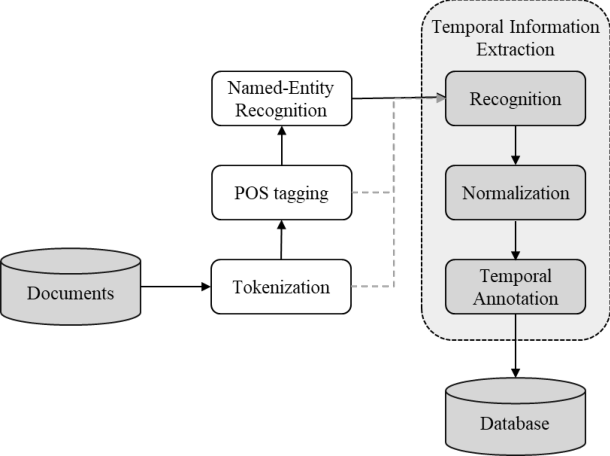
\includegraphics[width=1\textwidth]{标注过程.pdf}
    \caption{时间表达式标注过程}
    \label{fig:tagging_pregress}
\end{figure}

完整的时间信息抽取过程通常采用时间标注器(temporal tagger)完成,依照基于规则(rule-based)或基于语法(grammar-based)的方法进行标注。
一般地,标注器所使用的规则和语法由领域专家手工撰写(hand-driven),编写并扩展的代价较高,而由于时间信息高度依赖于语言的特性,解决方案通常是为一类语言或一种领域单独设计时间标注器。
除手工驱动外,时间信息抽取遇到的挑战还有判断文档创建时间(作为上下文锚时间)、界定(确定时间表达式在文本中的界限)、分类和规范化时间表达式、识别事件以及判断时间对象之间的时序关系。
此外,缺乏良好标注的包含时间信息的语料也是一个问题。从语言学的角度来看,时间表达式可以在不同的语言中以不同的形式表述,而语言本身的特性和某些歧义性使得时间信息抽取比词性标注(POS tagging, Part-Of-Speech tagging)任务困难的多。因此,开发一种通用的、跨领域、跨语言的时间标注器或标注系统比较困难。


\subsection{国内研究现状}

中文时间信息抽取语料较少,公开的测评数据集仅有采用Timex2与Timex3标注的ACE2005训练集与TempEval-2。
但这两个语料库含有的时间信息种类不够全、样本数不够多,故中文时间信息语料通常采用与自标注数据混合的形式构建,也导致目前可用时间标注器不多。
\citet{mingli2005ctemp}最早探索使用语法的方式来识别和归一化时间表达式,并采用启发式的规则解决时间信息间的语义冲突。

其后\citet{wu2005normalizing}在同一评测数据集上比较了基于机器学习的方式与基于语法的方式,发现对于中文时间信息抽取任务,基于机器学习方法不能达到与基于规则方法同样的效果。因此之后的中文时间信息抽取大多采用基于规则的形式。
FudanNLP\cite{qiu2013fudannlp}是最早通用的采用规则的时间标注器之一,但非专门处理时间抽取的工具,可用性欠佳。
\citet{li2014chinese}基于HeidelTime能够利用自动翻译和人工翻译的特性,将英语时间表达式自动翻译为中文并修正,在TempEval-3上取得了比较好的效果。
表~\ref{tab:research}列出了近十年中文时间信息抽取的一些研究。
\citet{liu2016cmedtex}考虑到临床上对于中文时间信息的需要,开发出一套基于规则的信息抽取系统,在ACE 2005上表现好于HeidelTime。

\begin{table}[h]
    \centering
    \caption{近十年中文时间信息抽取研究}
    \begin{tabular}{*{4}{c}}
        \toprule
        研究      & 任务        & 抽取方式 & 语料集   \\
        \midrule
        Liu(2016) & 识别+归一化 & 规则     & 自有语料 \\
        Liu(2015) & 识别+归一化 & 规则 & TempEval-2 \\
        Angeli and Uszkoreit(2013) & 识别 & 规则+机器学习 & ACE 2005 \\
        Wu(2010) & 识别 & 规则 & 自有语料 \\
        Wen(2010) & 归一化 & 规则 & ACE 2005\\
        He(2009) & 识别 & 规则+机器学习 & ACE 2005\\
        \bottomrule
    \end{tabular}
    \label{tab:research}
\end{table}


\subsection{国外研究现状}

##自然语言处理在每一个方向都发展出一套评价标准,时间抽取任务也不例外。
截止目前,在时间抽取任务语料库上达到SOTA(state-of-the-art)的时间标注器有:HeidelTime1\cite{strotgen2010heideltime},SuTime\cite{chang2012sutime},Chrono\cite{olex2018chrono}和ManTIME\cite{filannino2013mantime}。
时间标注器的评估标准在时间表达式的识别和归一化两方面有所不同,前者侧重于正确的识别文本中有关时间的片段,后者侧重于将时间表达式归一化到统一格式,其复杂程度取决于识别到的时间表达式的类型。
通用的评估方法是Fβ-measure,P(precision)为正确识别的时间表达式占总的识别出的时间表达式的相对频率,R(recall)为正确识别的时间表达式占文本中所有时间表达式的比例。

SuTime和HeidelTime都是基于规则(rule-based)开发的,前者由Stanford开发,对英语文本进行单独优化;后者由\citet{strotgen2010heideltime}开发,同时做到了跨语言(英语,德语,中文等)和跨领域(新闻与记叙文)的时间标注,其提出了一种自动翻译与人工标注相结合的方式,以解决跨领域、跨语言的时间信息抽取。
两者在TempEval-3上进行测评时都取得较好的表现。SuTime在时间表达式的识别上F1值为0.932,HeidelTime的F1值则为0.930(宽匹配)。
在时间表达式的归一化上HeidelTime更优,分数为0.86,而SuTime为0.75。

随着大数据时代的到来和计算力的提升,时间信息抽取系统也开始逐渐与机器学习、深度学习相结合,ClearTK\cite{bethard2013cleartk}采用支持向量机(SVM,support vector machine)与逻辑回归(LR,logistic regression)相结合的方式,在TempEval-3的整体分数为64。66。
ManTime\cite{filannino2013mantime}采用条件随机场(CRF,conditional random fields)与规则结合的方式,在TempEval-3上达到了68。97分,仅次于HeidelTime。

为了解决上文中提到的ISO-TimeML Timex3格式的局限性问题,\citet{laparra2018characters}于SemEval 2018 Task6中提出将SCATE作为Timex3格式的替代方案,以扩充之前标注格式的语义内容,使得时间抽取任务更偏向于语义分析任务,以增强机器学习方法在时间抽取任务上的表现。
此项赛事中,\citet{laparra2018characters}基于字符级别的神经网络到达了SOTA表现。但HeidelTime和Chrono也取得了较好的表现,说明基于规则的抽取方法仍大有可为。

\section{选题的先进性和实用性}

本文将语料中抽取到的时间信息分为以下几类:
\begin{enumerate}
    \item[(1)]  Datetime: 具体的时间日期,如‘2020年3月5日’;
    \item[(2)]  Datetime Interval: 两个Datetime形成的区间,如‘3月五日到六月7日’;
    \item[(3)]  Duration: 时长,如‘3天’;
    \item[(4)]  Duration Interval: 时长形成的区间,如‘3到五天’;
    \item[(5)]  Advanced features:
        \begin{enumerate}
            \item[(a)]  Frequency,如‘每两天’;
            \item[(b)]   Shift,如‘三天后’;
            \item[(c)]  Complex time expression,如‘明天下午三点到五点’;
            \item[(d)] Others。
        \end{enumerate}
\end{enumerate}

工业界落地的项目中,基本是采用规则的方式解决时间识别的问题,如阿里云小蜜(Alibaba ISR),百度unit(Baidu Unit)。
Facebook的Duckling同样采用PCFG识别时间表达式,但是对于某些时间表达式无法识别和归一化。表2做出了竞品分析,Frankenstein是本系统的名称。
以下各章节中若无特殊说明,均将‘中文时间信息抽取系统’默认为本项目中设计及开发的中文时间信息系统。
当时间信息作为系统完成某项任务的决策特征之一时,时间表达式识别的广度和归一化的正确度就显得十分必要。
本系统采用的方法应能显著改良中文时间信息抽取的体验。


\section{论文主要工作}

以作者所在的企业为例,智能客服是使用到实体解析功能的主营业务之一,主要为其他企业提供租车业务,是正常租车流程中人工客服的一种补充或直接替代。
系统需要从与客户的对话之中了解用户的意图,然后进行多轮对话,以完成一项任务的整体流程。时间信息抽取作为实体解析的一部分,是上层应用如知识图谱、填槽型多轮对话的基石,也是完成一项任务必不可少的内容。
中文时间信息抽取系统既可以作为中间件与其他信息处理模块协同工作处理完整的业务流程,又可作为单一的完整系统与用户直接实现交互。

本文将从以下几个方面阐述中文时间信息抽取系统的开发过程:
\begin{enumerate}
    \item[(1)] 时间表达式识别规则的设计和实现;
    \item[(2)] 时间表达式解析规则的设计和实现;
    \item[(3)] 用户调用接口的实现;
    \item[(4)] 用户交互界面的初步实现.
\end{enumerate}

整个项目进行过程中,本人的主要工作如下:
\begin{enumerate}
    \item[(1)] 参与时间表达式识别框架的构建和改进。将时间表达式的组合语义标注方式迁移到中文语境下,并设计时间归一化过程的表达式的计算;
    \item[(2)] 收集关于时间表达式的语料库,在现有中文时间表达式语料不完整、数据量不充足额情况下,对语料进行增强,并对语料加以整理和清洗;
    \item[(3)] 根据已有的一些类似的项目和相关的课题来构建中文时间信息抽取系统,优化基础设计方案然后对方案进行改进,并与过往的学界或工业界采取的方案进行比较测试,以评价中文时间信息抽取系统的性能;
    \item[(4)] 为方便测试与应用,配置用户交互界面,为用户提供灵活的识别方案。
\end{enumerate}


\section{本文的组织结构}

本文主要分为七个章节,没个章节的具体内容安排如下:

第一章: 绪论, 主要介绍时间表达式抽取的国内外发展状况,描述本文设计的代码检查工具的研究背景及其研究意义。

第二章: 相关知识与背景引导, 本章主要介绍了本项目中使用的相关技术及原理, 如概率无关上下文法、sklearn、MongoDB等.

第三章: 需求分析, 本章节从功能性需求和非功能性需求两个方面对本中文时间表达式信息抽取系统进行详尽的需求分析,分析总结了时间表达式信息抽取系统所需要实现的功能及其他性能需求。

第四章: 概要设计, 本章节主要介绍时间表达式信息抽取系统的框架设计和功能模块的设计, 详细的阐述了时间表达式信息抽取系统所应用的解决方案以及该系统的不同模块之间的协作.

第五章: 详细设计, 本章节对时间表达式信息抽取系统进行详细设计, 并介绍部分时间表达式识别和解析规则的具体实现.

第六章: 系统的测试与分析, 本章节主要是对系统的功能及性能进行评估, 确保本文的时间表达式信息抽取系统能够基本满足用户的各种需求,

第七章: 总结与张望. 本章节首先对七个月左右的实习工作和论文进行简单的总结, 同时对本文的时间表达式信息抽取系统中存在的不足进行描述分析, 且对本系统的未来发展进行展望, 提出对未来工作的优化建议.




